\documentclass{article}
\usepackage{geometry}
\usepackage{titling}
\usepackage{hyperref}
\usepackage{amsmath}
\usepackage{amssymb}
\usepackage{graphicx}
\usepackage{caption}
\usepackage{subcaption}
\usepackage{stmaryrd}
\usepackage{enumitem}
\usepackage[dvipsnames]{xcolor}

\geometry{
  a4paper,
  total = {170mm, 257mm},
  left = 20mm,
  top = 20mm,
}
\graphicspath{ {./images/} }

\newcommand{\addfig}[2]{\begin{figure}[!htb] \centering \includegraphics[width=#1\textwidth]{#2}\end{figure}}

\newcommand{\aexp}[1]{\langle\text{#1}\rangle}
\newcommand{\intexp}{\aexp{intexp}}
\newcommand{\var}{\aexp{var}}
\newcommand{\assert}{\aexp{assert}}
\newcommand{\sem}[1]{\left\llbracket #1\right\rrbracket}

\newcommand{\N}{\mathbb{N}}
\newcommand{\Z}{\mathbb{Z}}
\newcommand{\B}{\mathbb{B}}

\newcommand{\supr}{\bigsqcup\limits}

\title{Trabajo práctico N° 3}
\author{Emanuel Nicolás Herrador}
\date{Abril 2025}

\makeatletter
\def\@maketitle{%
  \newpage
  \null
  \vskip 1em%
  \begin{center}%
  \let \footnote \thanks
    {\LARGE \@title \par}%
    \vskip 1em%
    {\large \@date}%
  \end{center}%
  \par
  \vskip 1em}
\makeatother

\begin{document}

\maketitle

\noindent\begin{tabular}{@{}ll}
	Estudiante & \theauthor \\
\end{tabular}

\section*{Ejercicio 1}
Queremos ver si varios órdenes parciales son predominios o dominios.
Recordemos que un predominio es un orden parcial tal que toda cadena interesante tiene supremo, y que un dominio es un predominio con mínimo.

Ahora, si vemos cada uno de los órdenes parciales, tenemos:
\begin{enumerate}[label=(\alph*)]
	\item $\intexp$ con el orden discreto: es predominio al no tener cadenas interesantes.
	      No es dominio porque no tiene mínimo.
	\item $\intexp \to \B_\bot$: Veamos que $\B_\bot$ es un dominio dado que al ser orden llano no tiene cadenas interesantes y, además, tiene un mínimo.
	      Como $\B_\bot$ es un dominio, entonces $\forall A,\ A \to \B_\bot$ es un dominio.
	      Esto sucede porque para $f, g \in A \to \B_\bot,\ f \leq g \iff (\forall x,\ f(x) \leq g(x))$, por lo que los maximales son $f_0(x) = 0,\ f_1(x) = 1\ \forall x$ y el mínimo es $f_\bot(x) = \bot\ \forall x$.
	\item $\B_\bot \to \intexp$: Por $(a)$ sabemos que $\intexp$ es un predominio.
	      Bajo la misma idea realizada con el dominio, podemos llegar a que $\forall A,\ A \to \intexp$ es un predominio pero no un dominio dado que no existe un mínimo.
\end{enumerate}

\section*{Ejercicio 2}
Evito realizar el diagrama del dominio $(e)$ dado que es grande.
Respecto a lo demás, tenemos:
\begin{figure}[!htb]
	\centering
	\begin{subfigure}[b]{0.15\textwidth}
		\centering
		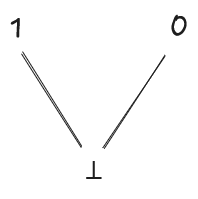
\includegraphics[width=\textwidth]{03-02-a.png}
		\caption{}
	\end{subfigure}
	\hfil
	\begin{subfigure}[b]{0.3\textwidth}
		\centering
		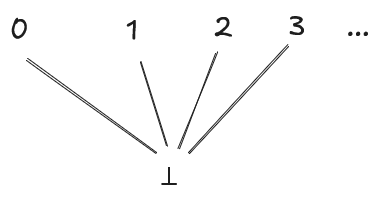
\includegraphics[width=\textwidth]{03-02-b.png}
		\caption{}
	\end{subfigure}
	\hfil
	\begin{subfigure}[b]{0.4\textwidth}
		\centering
		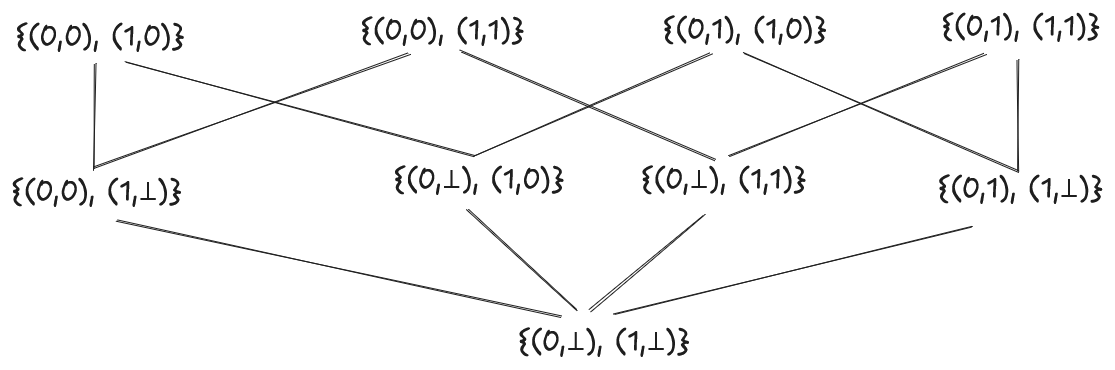
\includegraphics[width=\textwidth]{03-02-c.png}
		\caption{}
	\end{subfigure}
	\hfil
	\begin{subfigure}[b]{0.05\textwidth}
		\centering
		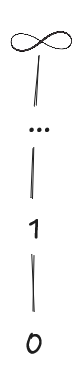
\includegraphics[width=\textwidth]{03-02-d.png}
		\caption{}
	\end{subfigure}
\end{figure}

\section*{Ejercicio 3}
Tenemos que indicar el menor elemento para cada dominio de los ejercicios anteriores.
Para ello, veamos que:
\begin{itemize}
	\item Para $\intexp \to \B_\bot$ es $f(x) = \bot\ \forall x \in \intexp$.
	\item Para $\B_\bot$ es $\bot$.
	\item Para $\N_\bot$ es $\bot$.
	\item Para $\B \to \B_\bot$ es $f(x) = \bot\ \forall x \in \B$.
	\item Para $\N^\infty$ es $0$.
	\item Para $\N^\infty \to \N^\infty$ es $f(x) = 0\ \forall x \in \N^\infty$.
\end{itemize}

\section*{Ejercicio 4}
Ahora, se pretende calcular el supremo de los siguientes conjuntos.
Para mayor comodidad, veamos cada ítem por separado.

\subsection*{Item A}
Tenemos $\mathcal{A} = \{n \in \N : n \text{ es par}\} \subseteq \N_\bot$.
Claramente no tiene supremo porque no tiene cota suprerior.
Esto se puede demostrar por absurdo, dado que sea $x \in \mathcal{A}$ el supruesto supremo, $x < x+2$ y $x+2 \in \mathcal{A}$.

\subsection*{Item B}
Tenemos $\mathcal{A} = \{n \in \N : n \text{ es par}\} \subseteq \N^\infty$.
La única cota suprerior de $\mathcal{A}$ es $\infty$, por lo que este elemento es claramente el supremo.

\subsection*{Item C}
Tenemos $\mathcal{A} = \{n \in \N : n \text{ es primo}\} \subseteq \N^\infty$.
De forma análoga a la anterior, el supremo es $\infty$.

\subsection*{Item D}
Tenemos $\mathcal{A} = \{V, F\} \subseteq \B_\bot$.
No tiene supremo porque es un orden llano.

\subsection*{Item E}
Tenemos $\mathcal{F} = \{f_n : n \in \N\} \subseteq \N \to \N_\bot$ donde:
\begin{equation*}
	f_n x = \begin{cases}
		1    & \text{si} x|n \\
		\bot & \text{cc.}
	\end{cases}
\end{equation*}

Para ello, notemos que $\forall x, i \in \N,\ f_i x \leq 1$.
Una cota suprerior es, entonces, la función constante $1$ ($C_1$) tal que $\forall x \in \N, C_1 x = 1$.

suprongamos, ahora, que $\exists g \in \N \to \N_\bot : g \leq C_1 \land (\forall f_i \in \mathcal{F},\ f_i \leq g)$.
Como $g \leq C_1$, entonces $\exists x \in \N : g(x) = \bot$.
Luego, no se cumple que $f_x \leq g$ dado que como $x|x$, entonces $f_x x = 1$ pero $g x = \bot$.
Por ello, demostramos por absurdo que no existe otra función $g$ menor a $C_1$ que sea cota suprerior de $\mathcal{F}$.

Finalmente, se demuestra que $C_1$ es supremo de $\mathcal{F}$.

\subsection*{Item F}
Tenemos $\mathcal{F} = \{f_n : n \in \N\} \subseteq \N \to \N_\bot$ donde:
\begin{equation*}
	f_n x = \begin{cases}
		x    & \text{si } |x-10| < \log(n + 1) \\
		\bot & \text{cc.}
	\end{cases}
\end{equation*}

Como $\forall x, i \in \N,\ f_i x \leq x$, entonces una cota suprerior es la función identidad ($I$) tal que $I(x) = x\ \forall x \in \N$.
suprongamos, ahora, que $\exists g \in \N \to \N_\bot : g \leq I \land (\forall f_i \in \mathcal{F},\ f_i \leq I)$.
Como $g \leq I$, entonces $\exists x \in \N : g(x) = \bot$.
Digamos $x \in \N : g(x) = \bot$.
Luego, no se cumple que $f_{e^{|x-10|}} \leq g$ porque:
\begin{equation*}
	\begin{aligned}
		|x-10|     & < \log(e^{|x-10|} + 1)     \\
		           & \Updownarrow               \\
		e^{|x-10|} & < e^{\log(e^{|x-10|} + 1)} \\
		           & \Updownarrow               \\
		e^{|x-10|} & < e^{|x-10|} + 1
	\end{aligned}
\end{equation*}
lo que significa que $f_{e^{|x-10|}} x = x$.
Finalmente, se llega a un absurdo que vino de suproner que existe una cota suprerior a $\mathcal{F}$ menor a $I$.

Por ello mismo, entonces, $I$ es el supremo de $\mathcal{F}$.

\section*{Ejercicio 5}
Recordemos las definiciones de cada propiedad de función.
Sean $P, Q$ predominios, $f \in P \to Q$ es monótona si $\forall x, y \in P,\ (x \leq y \Rightarrow fx \leq fy)$.
Decimos que $f$ es continua si para toda cadena $p_0 \leq p_1 \leq \dots$ el supremo $\bigsqcup\limits_{i \in \N} f_{p_i}$ existe y $\bigsqcup\limits_{i \in \N} f_{p_i} = f\left(\bigsqcup\limits_{i \in \N} p_i\right)$.

Ahora, sean $D, D'$ dominios con mínimos $\bot, \bot'$, entonces $f \in D \to D'$ es estricta si $f \bot = \bot'$.

Teniendo esto en cuenta, veamos ejemplos para cada espacio de función:
\begin{enumerate}[label=(\alph*)]
	\item Considerando $\B_\bot \to \B_\bot$, al ser $\B_\bot$ finito, si $f$ es monótona entonces tiene que ser continua ya que al preservarse las cadenas y ser todas no interesantes, se preservan también los supremos.
	      Respecto a una función continua y estricta, podemos considerar a $C_\bot$ dado que se mantiene el mínimo.

	\item Considerando $\N_\bot \to \N_\bot$, como se vio antes, sea $f$ una función monótona, como toda cadena de $\N_\bot$ es no interesante, se preservan también los supremos por lo que $f$ es también continua.
	      Respecto a una función continua y estricta, podemos considerar a $C_\bot$ dado que se mantiene el mínimo.

	\item Considerando $\N^\infty \to \N_\bot$, una función monótona pero no continua es $f_1 = \{(0, \bot), (1, \bot), \dots, (\infty, 0)\}$ dado que para la cadena $0 \leq 1 \leq \dots$ tenemos que $\bigsqcup\limits_{i \in \N} fi = \bot \neq f\left(\bigsqcup\limits_{i \in \N} i\right) = f \infty = 0$.
	      Respecto a una función continua y estricta, podemos considerar a $C_\bot$ dado que se mantiene el mínimo.

	\item Considerando $\N^\infty \to \N^\infty$, una función monótona pero no continua es $f_1 = \{(0, 0), (1, 0), \dots, (\infty, 1)\}$ dado que para la cadena $0 \leq 1 \leq \dots$ tenemos que $\bigsqcup\limits_{i \in \N} fi = 0 \neq f\left(\bigsqcup\limits_{i \in \N} i\right) = f \infty = 1$.
	      Respecto a una función continua y estricta, podemos considerar a $C_0$ dado que se mantiene el mínimo.
\end{enumerate}

\section*{Ejercicio 6}
Ahora, queremos caracterizar todas las funciones continuas en los espacios de funciones considerados en el ejercicio anterior.
Para ello, veamos cada una por separado:
\begin{enumerate}[label=(\alph*)]
	\item Considerando $\B_\bot \to \B_\bot$, como todas las cadenas son no interesantes entonces toda función monótona mantiene el supremo.
	      Luego, las funciones continuas son aquellas que mantienen el orden.
	      Por ello, el conjunto es $\left(\bigcup\limits_{x \in \B_\bot} C_x\right) \cup \{f : f \bot = \bot\}$.

	\item Considerando $\N_\bot \to \N_\bot$, al tener solo cadenas no interesantes, toda función monótona mantiene el supremo.
	      Con ello, un análisis similar al anterior nos lleva a que el conjunto de funciones continuas es $\left(\bigsqcup\limits_{x \in \N_\bot} C_x\right) \cup \{f : f \bot = \bot\}$.

	\item Considerando $\N^\infty \to \N_\bot$, la única cadena a tomar en cuenta para saber cuáles funciones monótonas no son continuas es $0 \leq 1 \leq \dots$.
	      Dada esa cadena, una función $f$ es continua si $\bigsqcup\limits_{i \in \N} f i = f\left(\bigsqcup\limits_{i \in \N} i\right) = f \infty$.
	      Luego, entonces, el conjunto de funciones continuas es $\left(\bigcup\limits_{x \in \N_\bot} C_x\right) \cup \{f : \exists x, y \in \N : (\forall k < x,\ f k = \bot) \land (\forall k \geq x,\ f k = y) \land f \infty = y \}$

	\item Considerando $\N^\infty \to \N^\infty$, del mismo modo que antes, la única cadena a considerar para ver qué funciones monótonas son no continuas es $0 \leq 1 \leq \dots$.
	      Por ello, buscamos que $f$ cumpla que sea monótona y $\supr_{i \in \N} f i = f\left(\supr_{i \in \N} i\right) = f \infty$.
	      Luego, entonces, el conjunto de funciones continuas es $\left(\bigcup\limits_{x \in \N^\infty} C_x\right) \cup \{f : f \text{ es monótona } \land \exists x \in \N^\infty : (\exists y \in \N : f(y) = x) \land (\forall y \leq x,\ f(y) \leq x) \land f \infty = x\}$
\end{enumerate}

\section*{Ejercicio 7}
Si ahora queremos reducir los conjuntos caracterizados de funciones continuas en el ejercicio anterior, entonces tendremos para cada caso lo siguiente:
\begin{enumerate}[label=(\alph*)]
	\item $\{f : f \bot = \bot\}$.
	\item $\{f : f \bot = \bot\}$.
	\item $\{C_\bot\} \cup \{f : f 0 = \bot \land \exists x, y \in \N : (\forall k < x,\ f k = \bot) \land (\forall k \geq x,\ f k = y) \land f \infty = y\}$.
	\item $\{C_\bot\} \cup \{f \text{ es monótona } \land \exists x \in \N^\infty : (\exists y \in \N : f(y) = x) \land (\forall y \leq x,\ f(y) \leq x) \land f \infty = x \land f 0 = 0\}$.
\end{enumerate}

\section*{Ejercicio 8}
Como se quiere caracterizar los puntos fijos y decidir cuál es el menor, recordemos primero al \textbf{Teorema del Menor Punto Fijo}.
Este expresa que sea $D$ un dominio y $F \in D \to D$ continua, entonces $\supr_{i \in \N} F^i \bot$ existe y es el menor punto fijo de $F$.

Ahora, veamos cada una de las funciones a considerar separadas por items.

\subsection*{Item A}
Consideramos $f : \N \to \N$ tal que $f n = n$.
Claramente, $\N$ es el conjunto de puntos fijos dado que incluso $f$ se define de ese modo.
Por ello, el menor punto fijo es $0$.

\subsection*{Item B}
Consideramos $h : \N^\infty \to \N^\infty$ tal que $h n = n + 1$.
Digamos que $x \in \N$, luego $h x = x + 1 \neq x$ por lo que no es punto fijo.
El caso de $\infty$ es diferente dado que $\infty + 1 = \infty$, por lo que es el único punto fijo de $h$.

\subsection*{Item C}
Consideramos $g : \intexp \to \intexp$ tal que $g e = e$.
Notemos que, de la misma forma que $(a)$, todo elemento de $\intexp$ un punto fijo.
Lo que resta ver es cuál es el mínimo entre estos.
Como no existe este mínimo dado que $\intexp$ es un orden discreto, entonces no existe un mínimo punto fijo.

\subsection*{Item D}
Consideramos $k : \N^\infty \to \N^\infty$ tal que:
\begin{equation*}
	k n = \begin{cases}
		n + 1 & \text{ si } n < 8 \\
		n     & \text{ cc. }
	\end{cases}
\end{equation*}

Claramente, entonces, los puntos fijos son caracterizados dentro de este conjunto: $\{x \in \N : x \geq 8\}$.
Por ello, también, el menor punto fijo es $8$.

\section*{Ejercicio 9}
Vamos a tomar cada función $F$ como un caso aparte para mayor comodidad a la hora de realizar la solución a este ejercicio.

\subsection*{Item A}
Consideramos $F \in (\N \to \N_\bot) \to (\N \to \N_\bot)$ tal que:
\begin{equation*}
	F f = \begin{cases}
		f                     & \text{ si } f \text{ es una función total} \\
		\bot_{\N \to \N_\bot} & \text{ cc. }
	\end{cases}
\end{equation*}

Por definición, $f$ es una función total si para todo elemento de $\N$ está definida.
Es decir, básicamente es función total si su imagen no contiene a $\bot$.

Ahora, si consideramos la cadena de funciones $f_0 \leq f_1 \leq \dots$ donde:
\begin{equation*}
	f_i x = \begin{cases}
		x    & \text{ si } x \leq i \\
		\bot & \text{ cc. }
	\end{cases}
\end{equation*}
tenemos que $\supr_{i \in \N} F f_i = \supr_{i \in \N} \bot_{\N \to \N_\bot} = \bot_{\N \to \N_\bot}$ dado que $f_i$ es una función parcial.
Sin embargo, $F\left(\supr_{i \in \N} f_i\right) = F I = I$ donde $I$ es la función identidad.
Por ello, entonces, al no ser igual el supremo tenemos que $F$ no es continua.

Como segunda parte, entonces, vamos a calcular $F^{(i)} \bot_{\N \to \N_\bot}$ para $i = 0, 1, 2$.
Luego, veamos:
\begin{equation*}
	\begin{aligned}
		F^0 \bot_{\N \to \N_\bot} & = \bot_{\N \to \N_\bot}                        \\
		\\
		F^1 \bot_{\N \to \N_\bot} & = F \bot_{\N \to \N_\bot}                      \\
		                          & = \begin{cases}
			                              \bot_{\N \to \N_\bot} & \text{ si es total } \\
			                              \bot_{\N \to \N_\bot} & \text{ cc. }
		                              \end{cases} \\
		                          & = \bot_{\N \to \N_\bot}                        \\
		\\
		F^2 \bot_{\N \to \N_\bot} & = F F \bot_{\N \to \N_\bot}                    \\
		                          & = F \bot_{\N \to \N_\bot}                      \\
		                          & = \bot_{\N \to \N_\bot}
	\end{aligned}
\end{equation*}

\subsection*{Item B}
Ahora, consideramos la función $F \in (\N \to \N_\bot) \to (\N \to \N_\bot)$ tal que:
\begin{equation*}
	F f n = \begin{cases}
		0        & \text{ si } n = 0 \\
		f(n - 2) & \text{ cc. }
	\end{cases}
\end{equation*}

Para ver que $F$ es continua, queremos demostrar que dada una cadena $f_0 \leq f_1 \leq \dots$ entonces $\supr_{i \in \N} F f_i = F\left(\supr_{i \in \N} f_i\right)$.

Sin embargo, primero demostraremos que $F$ es monótona para que sea más sencillo hacer la demostración de continuidad.
Para ello, consideremos $f, g \in \N \to \N_\bot : f \leq g$.
Por definición, entonces, $\forall x \in \N,\ f x \leq g x$.
Luego, si $n = 0$ tenemos que $F f 0 = 0$ y que $F g 0 = 0$ por lo que se cumple la desigualdad en este caso.
Ahora, si $n \neq 0$ tenemos que $F f n = f(n-2)$ y que $F g n = g(n-2)$.
Como $f \leq g$, entonces $f(n-2) \leq g(n-2)$ por lo que se cumple para este otro caso.
Finalmente, $F$ es monótona. $\blacksquare$

Respecto a la continuidad, vamos a demostrarlo según el valor de $n$.
Digamos que $n = 0$, entonces:
\begin{equation*}
	\begin{aligned}
		\left(\supr_{i \in \N} F f_i\right) 0 & = \supr_{i \in \N} F f_i 0 \\
		                                      & = \supr_{i \in \N} 0       \\
		                                      & = 0                        \\
		\\
		F\left(\supr_{i \in \N} f_i\right) 0  & = 0
	\end{aligned}
\end{equation*}
por lo que se cumple la igualdad en este caso.

Ahora, digamos $n \neq 0$:
\begin{equation*}
	\begin{aligned}
		\left(\supr_{i \in \N} F f_i\right) n & = \supr_{i \in \N} F f_i n                  \\
		                                      & = \supr_{i \in \N} f_i(n - 2)               \\
		\\
		F\left(\supr_{i \in \N} f_i\right) n  & = \left(\supr_{i \in \N} f_i\right) (n - 2) \\
		                                      & = \supr_{i \in \N} f_i(n - 2)
	\end{aligned}
\end{equation*}
por lo que se cumple la igualdad aquí también.

Luego, entonces, se demuestra que dada una cadena entonces el supremo se conserva por lo que $F$ es continua. $\blacksquare$

Como segunda parte, ahora vamos a calcular $F^{(i)} \bot_{\N \to \N_\bot}$ para $i = 0, 1, 2$.
Luego, veamos:
\begin{equation*}
	\begin{aligned}
		F^0 \bot_{\N \to \N_\bot} n & = \bot_{\N \to \N_\bot}                        \\
		\\
		F^1 \bot_{\N \to \N_\bot} n & = F \bot_{\N \to \N_\bot} n                    \\
		                            & = \begin{cases}
			                                0                     & n = 0        \\
			                                \bot_{\N \to \N_\bot} & \text{ cc. }
		                                \end{cases}         \\
		\\
		F^2 \bot_{\N \to \N_\bot} n & = F F \bot_{\N \to \N_\bot} n                  \\
		                            & = \begin{cases}
			                                0                             & n = 0        \\
			                                F \bot_{\N \to \N_\bot} (n-2) & \text{ cc. }
		                                \end{cases} \\
		                            & = \begin{cases}
			                                0                     & n = 0        \\
			                                0                     & n-2 = 0      \\
			                                \bot_{\N \to \N_\bot} & \text{ cc. }
		                                \end{cases}         \\
		                            & =\begin{cases}
			                               0                     & n \in \{0, 2\} \\
			                               \bot_{\N \to \N_\bot} & \text{ cc. }
		                               \end{cases}
	\end{aligned}
\end{equation*}

\section*{Ejercicio 10}
Queremos calcular la menor función $f \in \Z \to \Z_\bot$ que satisface
\begin{equation*}
	f n = \begin{cases}
		1            & n = 0    \\
		n * f(n - 1) & n \neq 0
	\end{cases}
\end{equation*}

Para ello, deberemos usar el Teorema del Menor Punto Fijo para $F : (\Z \to \Z_\bot) \to (\Z \to \Z_\bot)$ tal que
\begin{equation*}
	F f n = \begin{cases}
		1            & n = 0    \\
		n * f(n - 1) & n \neq 0
	\end{cases}
\end{equation*}
por lo que voy a demostrar primero que $F$ es monótona y, luego, que es continua.

Vamos a demostrar que $F$ es monótona.
Para ello, digamos $f, g \in \Z \to \Z_\bot : f \leq g$.
Esto quiere decir que $\forall x \in \Z,\ f x \leq g x$.
Si $n = 0$, $F f 0 = 0 \leq F g 0 = 0$.
Si $n \neq 0$, $F f n = n * f(n - 1) \leq F g n = n * g(n - 1)$ dado que $f(n - 1) \leq g(n - 1)$.
Luego, entonces, $F$ es monótona. $\blacksquare$

Ahora, vamos a demostrar que $F$ es continua.
Para ello, digamos que tenemos la cadena $f_0 \leq f_1 \leq \dots \leq f_n \leq \dots$ de $\Z \to \Z_\bot$.
Queremos ver que $\left(\supr_{i \in \N} F f_i\right) = F\left(\supr_{i \in \N} f_i \right)$.
Para ello, vamos a verlo para cada $n \in \Z$.
Si $n = 0$:
\begin{equation*}
	\begin{aligned}
		\left(\supr_{i \in \N} F f_i\right) 0 & = \supr_{i \in \N} F f_i 0 \\
		                                      & = \supr_{i \in N} 1        \\
		                                      & = 1                        \\
		\\
		F\left(\supr_{i \in \N} f_i\right) 0  & = 1
	\end{aligned}
\end{equation*}
entonces se cumple la igualdad.
Ahora, si $n \neq 0$:
\begin{equation*}
	\begin{aligned}
		\left(\supr_{i \in \N} F f_i\right) n & = \supr_{i \in \N} F f_i n                     \\
		                                      & = \supr_{i \in \N} (n * f_i(n - 2))            \\
		                                      & = n * \supr_{i \in \N} f_i(n - 2)              \\
		\\
		F\left(\supr_{i \in \N} f_i\right) n  & = n * \left(\supr_{i \in \N} f_i\right)(n - 2) \\
		                                      & = n * \supr_{i \in \N} f_i(n - 2)
	\end{aligned}
\end{equation*}
entonces se cumple la igualdad.
Por ello, finalmente, se demuestra que $F$ es continua. $\blacksquare$

Finalmente, entonces, ya estamos habilitados para usar el Teorema del Menor Punto Fijo.
Para ello, primero veamos algunos casos para $F^{(i)} \bot$:
\begin{equation*}
	\begin{aligned}
		F^0 \bot n & = \bot                               \\
		\\
		F^1 \bot n & = F \bot n                           \\
		           & = \begin{cases}
			               1               & n = 0        \\
			               n * \bot(n - 1) & \text{ cc. }
		               \end{cases}     \\
		           & = \begin{cases}
			               1    & n = 0        \\
			               \bot & \text{ cc. }
		               \end{cases}                \\
		\\
		F^2 \bot n & = F F \bot n                         \\
		           & = \begin{cases}
			               1                  & n = 0        \\
			               n * F \bot (n - 1) & \text{ cc. }
		               \end{cases}  \\
		           & = \begin{cases}
			               1     & n = 0        \\
			               n * 1 & n-1 = 0      \\
			               \bot  & \text{ cc. }
		               \end{cases}               \\
		           & = \begin{cases}
			               1    & n = 0        \\
			               n    & n = 1        \\
			               \bot & \text{ cc. }
		               \end{cases}                \\
		\\
		F^3 \bot n & = F F^2 \bot n                       \\
		           & = \begin{cases}
			               1                   & n = 0        \\
			               n * F^2 \bot(n - 1) & \text{ cc. }
		               \end{cases} \\
		           & = \begin{cases}
			               1         & n = 0        \\
			               n         & n-1 = 0      \\
			               n * (n-1) & n-1 = 1      \\
			               \bot      & \text{ cc. }
		               \end{cases}           \\
		           & = \begin{cases}
			               1           & n = 0        \\
			               n           & n = 1        \\
			               n * (n - 1) & n = 2        \\
			               \bot        & \text{ cc. }
		               \end{cases}
	\end{aligned}
\end{equation*}

Observando esto, propongo que $F^{(i)} \bot$ es igual a:
\begin{equation*}
	F^{(i)} \bot n = \begin{cases}
		n!   & 0 \leq n < i \\
		\bot & \text{ cc. }
	\end{cases}
\end{equation*}

Viendo que el caso base se cumple, suponemos la hipótesis para $k \in \N$ y queremos verlo para $k+1$ así lo demostramos por inducción:
\begin{equation*}
	\begin{aligned}
		F^{k+1} \bot n & = F F^k \bot n                      \\
		               & = \begin{cases}
			                   1                  & n = 0        \\
			                   n * F^k \bot (n-1) & \text{ cc. }
		                   \end{cases} \\
		               & = \begin{cases}
			                   1          & n = 0          \\
			                   n * (n-1)! & 0 \leq n-1 < k \\
			                   \bot       & \text{ cc. }
		                   \end{cases}       \\
		               & = \begin{cases}
			                   1    & n = 0          \\
			                   n!   & 1 \leq n < k+1 \\
			                   \bot & \text{ cc. }
		                   \end{cases}             \\
		               & = \begin{cases}
			                   n!   & 0 \leq n < k+1 \\
			                   \bot & \text{ cc. }
		                   \end{cases}
	\end{aligned}
\end{equation*}
por lo que se demuestra por inducción esta forma para $F^{(i)}$. $\blacksquare$

Ahora, como el menor punto fijo es el supremo de esta cadena, tenemos que:
\begin{equation*}
	\left(\supr_{i \in \N} F^i \bot \right) n = \begin{cases}
		n!   & 0 \leq n     \\
		\bot & \text{ cc. }
	\end{cases}
\end{equation*}

\section*{Ejercicio 11}
Si queremos caracterizar las funciones que satisfacen la ecuación dada por:
\begin{equation*}
	f n = \begin{cases}
		f(n - 1)     & n < 0 \\
		1            & n = 0 \\
		n * f(n - 1) & n > 0
	\end{cases}
\end{equation*}
debemos tener en cuenta que si $n < 0$ entonces $f n = f(n-1) = f(n-2) = f(n-3) = \dots$ infinitamente.
Además, es claro que para $n \geq 0$ llegamos al mismo resultado obtenido en el ejercicio $10$.
Finalmente, entonces, se cumple que las funciones que satisfacen esta ecuación son de la forma:
\begin{equation*}
	f n = \begin{cases}
		k  & n < 0    \\
		n! & n \geq 0
	\end{cases}
\end{equation*}
para un $k \in \Z_\bot$.

Respecto a la comparación de esta ecuación con la del ejercicio 10, podemos ver que la del ejercicio anterior cumple la caracterización de este aunque no es la única.

\end{document}
